\documentclass[10pt]{article}
\usepackage[margin=0.9 in]{geometry}
\usepackage{amsmath, booktabs, hyperref, graphicx}
\title{Physical Action Effects in Dexterous Interaction Models:\\Measurement, Randomized Identification, and Task-Utility Prerequisites}
\author{Exploratory working manuscript, revision 10}
\date{2 October 2026}
\begin{document}
\maketitle
\begin{abstract}
Physical action prediction can support dexterous control only when executable
interventions are informative and their information improves task decisions.
We investigate these prerequisites on an existing Inspire-hand simulation
substrate, independently reconstructing actuator decoding, object geometry,
current-state inputs and sustained-holding labels. An initial replay procedure
fails strict pre-intervention matching; subsequent prospective randomization
avoids claims of cloned solver states. Several fresh action-effect and task
screens fail their fixed gates. We preserve a mismatch between original
25--36-frame lift references and longer holding criteria, and separately create
an explicitly synthetic 90-frame plateau task. A scratch reference-relative
absolute-target actor succeeds in 56/64 trials on one preselected motion but only
56/192 overall. A 6144-trajectory randomized support forecast improves strongly
against state-only prediction yet gains only 6.68\% over a strong motion/action
mean, failing its 10\% gate. The first actual matched feature-policy experiment
uses 9216 training and 1536 evaluation trajectories: all three learned variants
choose identical deterministic actions on every evaluated state, and the Cm
utility gate fails. Two further 1536-trajectory tests separately examine natural
slip feedback and selective independent-finger corrections; both fail their
prospective control gates. These results distinguish physical observability,
intervention feasibility and learned policy utility. They neither establish a
new general modeling method nor a universal impossibility result. A new
continuous-action auxiliary-critic comparison has passed engineering and one
training-update audit but remains incomplete, with no prospective utility result.
All original failed gates, privileged-state limitations and synthetic task
boundaries are retained. Validation across training seeds, generalization,
hardware evidence and journal readiness remain unestablished.
\end{abstract}

\section{Problem and relation to prior work}
An interaction model can fit common motion while failing to compare alternative actions.
Useful comparisons additionally require experiments capable of measuring physical
differences at the states in which actions are selected. We examine this prerequisite
alongside bounded policy-initializer checks. The repository provides self-trained
actors, geometric models and a DExplore simulation substrate \cite{xu2025}. Historical
policy audits are motivation rather than fresh evidence for this manuscript.

Shared particle actions and cross-embodiment world models already support planning
\cite{he2025}. Value-aware objectives \cite{farahmand2017}, predictor-level action
recovery \cite{qiu2026} and multi-step controllability representations \cite{rudolph2024}
are established. Contact-consistent replay and actuator residuals are also developed
by Contact-UAN \cite{fey2026}. Our small physical MLP studies do not reproduce these
systems or establish priority for their general principles. The present contribution
is an exploratory evidence record with frozen hypotheses and retained failures.
Recent tactile world models already forecast contact evolution: DexTacWAM models
joint visual and tactile futures \cite{yuan2026}, while DexTouch-WM aligns human
and robot touch/action spaces and studies synthetic policy trajectories
\cite{qin2026}. WHIRL predicts future human-intervention probability and shapes
actor risk \cite{yin2026}. Generic contact forecasting or predictive risk shaping
therefore cannot provide a new claim for this project. These primary sources
are literature context, not reproduced baselines.
WorldSimProbe already formalizes action realization and grounded environment
response requirements through controlled simulator evaluation \cite{co2026}.
Facet-0 combines action-wrench prediction, a contact-aware critic and reinforcement
learning adaptation \cite{deng2026}. Generic physical grounding diagnostics or
valuing contact consequences therefore cannot constitute our novelty. Our witness
and baseline-learning tests identify experimental prerequisites, not a competing
foundation model. Full methodological comparisons remain necessary.

\section{Initial physical and contrast-learning screens}
Four panels combine actor seeds 286/287 with environment seeds 288/289, each with
32 environments for each of three airplane motions. A retrospective trigger schedules
one step after the first reference event where independent hand and object force
proxies are active. A one-step wrist-z action change requests a plus or minus 10-mm
PD target offset. This is a desired offset, not measured wrist travel. All subsequent
normalized actions and RNG schedules are replayed. Two zero arms measure repeated
process variation. Each object response subtracts its own actual pre-intervention
position. Pulse and repeat contrasts are summarized by vector RMS.

\begin{table}[h]
\centering
\begin{tabular}{lrr}
\toprule
Steps & Pulse RMS (mm) & Repeat RMS (mm)\\
\midrule
1 & 1.914 & 0.000\\
2 & 2.572 & 0.084\\
5 & 7.150 & 0.101\\
10 & 18.827 & 0.444\\
20 & 75.463 & 6.081\\
30 & 105.792 & 9.638\\
\bottomrule
\end{tabular}

\caption{Initial fixed panels: pulse versus observed zero-repeat position contrasts.}
\end{table}

At five and ten steps, contrast ratios are 70.44 and 42.36. At one step, the observed
zero repeat is exactly zero; its ratio is undefined rather than made finite by an
arbitrary denominator. Mixed vertical signs fail the joint physical gate. No beneficial
lifting or population confidence bound follows from a large observed contrast.

The subsequent vector-learning decision retains this failure. It fits 192 actor-286
windows and tests 192 actor-287 windows using four past/current physical states and
ten preset replay actions. Future observed physical states are absent from inputs.
Matched two-layer 128-unit SiLU networks predict five/ten-step position responses;
three seeds each receive 1000 Adam updates. Differential training adds measured
plus--minus contrast loss. All normalization uses fit rows. Fixed test panels were
already inspected by the physical experiment, making this reused-data exploration.

\begin{table}[h]
\centering
\begin{tabular}{lrr}
\toprule
Input/objective & Five steps (mm) & Ten steps (mm)\\
\midrule
Factual & 10.121 & 26.546\\
Differential & 10.114 & 26.990\\
No pulse & 9.922 & 26.456\\
Global fit mean & 10.061 & 26.259\\
Motion fit mean (privileged) & 10.137 & 26.340\\
\bottomrule
\end{tabular}

\caption{Actor-transfer contrast RMSE, millimeters; learned rows average three optimization seeds.}
\end{table}

Differential training does not improve over factual or global fit-mean controls.
Vertical sign agreement is 32.6\%/31.1\%, below its fixed 75\% gate. Both initial
screens are UNPROMISING. Increasing steps or choosing another seed is not used to
salvage these exact designs. Physical acquisition took 481.9 seconds; fitting took
17.2 seconds on one RTX 3090.

\section{Geometry and larger archived predictive screen}
Full sampled current geometry places 318 of 384 old triggers within 20 mm. However,
actor 287's motion 1 is entirely outside that range in both old test panels, with
gaps 55--105 mm. Independent force proxies can both activate due to table contacts.
The geometric shift is documented, without identifying it as the sole cause of
learning failure or redefining the old gate.

We next use two immutable, episode-disjoint historical collections, 960 complete
episodes each. Nonterminal frames at step modulo 16 equal to zero yield 32902 fit
and 32896 test rows. These collections have been used by previous research and are
not pristine Validation data. The current-near test stratum contains 1756 frames
from 639 episodes; proximity uses a frozen stride-8 surface convention.

The target is one-step object-position residual over constant velocity, expressed
in the current object frame. State input includes joint angles and velocities,
object velocities, gravity direction, object height, palm/tip relative positions
and force proxies. Matched effect networks receive either zero action slots, native
commands, exact PD-target/FK palm-tip motion, predicted realized hand motion, or
measured future hand motion. The last is a privileged diagnostic. An independently
fit actuator model predicts joint residuals before the learned-motion variant's FK.
Effect networks have two 128-unit SiLU layers, fixed 1000 updates and three seeds.
Sampling is half-near and half-all fit rows. No test-selected checkpoint is used.

\begin{table}[h]
\centering
\begin{tabular}{lrr}
\toprule
Effect input & Near RMSE (mm) & All RMSE (mm)\\
\midrule
State only & 17.180 & 7.328\\
Native command & 16.436 & 7.330\\
Nominal PD motion & 14.599 & 7.093\\
Predicted hand motion & 15.066 & 7.206\\
Measured future hand (privileged) & 13.994 & 7.001\\
Passive & 23.400 & 7.587\\
\bottomrule
\end{tabular}

\caption{Archived one-step vector prediction error, seed-mean millimeters. Near and all-state strata differ.}
\end{table}

The predicted-motion primary method gains 8.33\% over command input, failing the
10\% requirement despite beating state-only, passive and its geometric transport
control. Its gate remains UNPROMISING. Actuator wrist-position errors are
11.75--12.07 mm near the object. Measured future hand motion includes possible
contact feedback and cannot establish a deployable causal mediator.

The separately reported nominal-motion variant gains 11.18\% and is better in each
seed. This motivates a separately frozen fresh causal test; it does not retroactively
replace the primary method. The label-free nominal no-slip transport control is
inaccurate, with near RMSE 133.64 mm. The full screen took 53.64 seconds. All 30
saved held RMSE metrics were independently recomputed.

\section{Fresh proximity acquisition and failed matching requirement}
New environment seeds 490/491 are combined with the same two actors. A compact
reference records up to 360 steps, stopping at the first native termination.
For each environment, acquisition selects the first pre-action step at or after
step 10 with five remaining nonterminal transitions, both current force proxies,
and full sampled surface distance at most 20 mm. Future object outcomes never
choose a trigger. Frozen assets provide 1538 hand and 1024 object points.

All 384 environments acquire a qualifying state, including all three motions in
every panel. The maximum sampled gap per panel is 16.60, 15.57, 18.83, 18.12 mm.
Eight cold processes per panel implement two zeros and one-step plus/minus pulses
in world x, y, z. Initial tensors, physical properties, actor/RMS states, actions and
RNG schedules are checked. Warm solver state is not asserted to be cloneable.
The existing effect models are frozen before acquisition; no refit is allowed.

The intended comparison requires pre-intervention position RMS at most 0.05 mm,
maximum joint difference at most 0.0001, and maximum quaternion-component difference
at most 0.0001. Joint coordinates combine translations in meters and angles in
radians; quaternion differences are dimensionless component differences.

\begin{table}[h]
\centering
\begin{tabular}{lrrr}
\toprule
Panel & Position RMS (mm) & Joint max & Quaternion max\\
\midrule
t286_s490 & 0.003554 & 0.0000732 & 0.0000670\\
t286_s491 & 0.010859 & 0.0002204 & 0.0006188\\
t287_s490 & 0.007110 & 0.0000000 & 0.0000416\\
t287_s491 & 0.013398 & 0.0000982 & 0.0000881\\
\bottomrule
\end{tabular}

\caption{Maximum pre-intervention mismatch over arms relative to zero-a. Limits: position 0.05 mm; joint and quaternion components 0.0001.}
\end{table}

All 32 physical arms complete, but seven arms of panel actor 286/seed 491 fail the
joint/orientation precondition. The first detected failure is zero-b, before any
action intervention. Execution stops with FAILED; the scientific transfer screen
is UNCLEAR due to invalid matching. No favorable arm or window is retained, no
threshold is widened, and no pooled causal score or model winner is reported.
Acquisition and the failed analysis took 1152.21 seconds. This is a measurement
blocker, not a refutation of the nominal predictor.

\section{Exact-null recovery mechanism screen}
Six native commands are overwritten by dependent finger targets. Randomizing them
leaves every PD target exactly unchanged; all 32896 held rows verify this bitwise.
We test whether recovering such independent null commands from model-generated
object predictions induces false action responses. A truthful physical transition
cannot recover an independent normalized null coordinate with population MSE below
one. This is an elementary conditional-variance bound, not a novel theorem.
Mutual-information sufficiency limits are already studied \cite{rakelly2021}.

Every minibatch independently randomizes null commands while keeping physical
labels fixed. Four matched physical predictors receive factual loss only, full
inverse loss, effective-command inverse loss, or hard-canonicalized forward input
with effective inverse loss. Inverse heads take current state and generated object
residuals, never actual future state. Seeds 511--513 each train for 1000 updates;
the auxiliary coefficient is fixed at one. Hard canonicalization guarantees null
invariance by construction, without establishing learned causal correctness.

\begin{table}[h]
\centering
\begin{tabular}{lrrr}
\toprule
Variant & Near RMSE (mm) & Null response (mm) & Null inverse MSE\\
\midrule
Factual only & 16.557 & 1.118 & not trained\\
Full inverse & 16.534 & 1.079 & 1.002\\
Effective inverse & 16.531 & 1.069 & 1.023\\
Hard quotient + inverse & 16.564 & 0.000 & 1.023\\
\bottomrule
\end{tabular}

\caption{Exact-null intervention diagnostics, near stratum and seed means. Untrained null-head coordinates in effective/quotient variants are diagnostic only.}
\end{table}

Full inverse null error remains near the population floor and its null response is
below factual-only in every seed. Three of five interference gates fail: UNPROMISING.
The proposed inverse-induced null-encoding mechanism is not supported here.
Hard canonicalization removes null response, with little factual-error change.
This screen took 33.06 seconds; 66 saved prediction/recovery metrics were independently
audited. It is neither an AD-WM reproduction nor a general rejection of inverse learning.

\section{Prospective randomized identification}
To avoid invalid cold-replay matching, we acquire a single factual transition
per independently assigned intervention. Four 768-environment panels combine
actors 286/287 with initial seeds 492/493, 256 environments per motion. Assignment
is drawn with a private CPU generator before physics. The trigger is the first
even current step at or after 10 with both force proxies and full sampled
hand--object gap at most 20 mm. A zero arm or one-step plus/minus wrist pulse in
world x, y, z is executed once; the actor remains closed loop. All 3072 windows
complete. Realized counts per motion are 37/37/37/37/36/36/36; recorded known
propensities account for the unequal count convention.

Let Y be observed one-step world position residual over current object velocity.
For each wrist axis j, define Z_j as the observed residual times the difference
between the inverse-propensity indicators for its plus and minus arms. Under
randomization and the independent-environment potential-outcome assumption,
its conditional mean is the plus-minus physical effect tau_j(X). For predictions
f, g, the row score is sum(f squared - g squared - 2(f-g)Z), summing all three
output coordinates and intervention axes. Its expectation is the squared
conditional-effect risk of f minus that of g. This elementary estimator identifies
a difference, not absolute effect RMSE or individually observed counterfactuals.
Weak numeric interactions between batched environments remain an assumption
limitation; exact solver-state cloning is not asserted.

Existing nominal-motion and command checkpoints 411--413 are frozen before the
trial. Each scores all six candidate commands at the same current context.
Per-model losses are averaged across seeds. Descriptive intervals use 2000
bootstrap replicates, preserving shared initial-seed/environment blocks across
actors within six initial-seed/motion strata.

\begin{table}[h]
\centering
\begin{tabular}{lrrr}
\toprule
Comparison & Point (mm^2) & Central95% & Upper95%\\
\midrule
nominal minus command & 0.122 & [-0.919,1.187] & 1.013\\
nominal minus zero & -0.326 & [-1.985,1.350] & 1.124\\
command minus zero & -0.448 & [-1.393,0.455] & 0.296\\
\bottomrule
\end{tabular}

\caption{Randomized held-window conditional-effect risk differences, mm squared; negative favors the first predictor.}
\end{table}

All three nominal-motion gates fail: UNPROMISING. Its historical 11.18 percent
factual error advantage does not establish causal action-effect superiority.
The trial takes 137.84 seconds after a retained 35.85-second device-alias engineering
failure. All 3072 physical windows, risk statistics and 107 input hashes pass an
independent numeric audit. We stop direct control use of these archived models.

\section{Direct randomized learning and strong controls}
The 3072 observed randomized windows now become fit data. A new test uses initial
seeds 494/495 and all 3072 windows; no future test outcome chooses a model. This
cohort changes the assignment protocol explicitly to independent seven-arm draws
with propensity 1/7, avoiding forced assignment balance. Counts are recorded as
realized; no rebalancing or partial-window selection is performed.

Context comprises 63 current physical/geometry features and 18 reference commands.
Six overwritten finger-command inputs are canonicalized to zero. Motion identity
and observed future states are excluded. Two nuisance folds separate acquisition
seeds 492/493, keeping shared actor/environment blocks together. Each nuisance
model predicts Y from context, scales only its own fit fold, and predicts the
other fold. Subtracting this out-of-fold response mean before constructing the
inverse-propensity pseudo-contrast preserves its conditional mean. Crossfitting
and randomization are established methods, not novelty claims.

For seeds 611--613, direct models have 81 inputs, 128/128 SiLU layers and nine outputs
reshaped as a world contrast matrix. Factual controls receive the same context
plus six pulse indicators and predict three world residual coordinates. All use
Adam 0.001, weight decay 0.0001, uniform 256-row minibatches and fixed final checkpoints.
Direct/factual/nuisance models get 1000 updates; the compute control gets 3000
factual updates, matching direct plus two nuisance update counts but not asserting
identical FLOPs or output capacity. All scales use fit rows only. A per-seed global
mean of residualized FIT contrasts and zero effect are additional strong controls.

Fresh test risk uses original observed residuals and known propensities, without
nuisance fitting on test. The gate requires a one-sided 95 percent upper risk bound
below zero against every control and favorable direct-minus-factual point in every
seed. Bootstrap preserves the same six paired strata as above.

\begin{table}[h]
\centering
\begin{tabular}{lrrr}
\toprule
Direct minus control & Point (mm^2) & Central95% & Upper95%\\
\midrule
factual & 23.977 & [2.024,48.106] & 44.201\\
factual compute matched & 24.278 & [2.370,48.434] & 44.586\\
global residualized & 20.820 & [-1.311,45.184] & 40.882\\
zero & 20.541 & [-1.223,45.436] & 40.638\\
\bottomrule
\end{tabular}

\caption{Direct randomized learner minus each frozen control, mm squared; every fixed gate fails.}
\end{table}

Direct-minus-factual seed points 32.35/19.35/20.23 all have the wrong direction.
The direct method is UNPROMISING and ends without extra updates or label clipping.
Fit/test take 30.31/134.49 seconds on separate admitted GPUs, producing 3.41/11.89 MiB.
Six nuisance-fold scales, 16 fit model/data files, held predictions, all risk arrays
and bootstrap intervals pass independent CPU/NumPy audits.

After retaining this primary failure, exploratory comparisons between the already
frozen controls suggest factual-minus-zero/global differences of-3.436/-3.158 mm
squared, with one-sided 95 percent upper bounds-1.106/-1.222. More factual updates
have no robust incremental advantage over 1000 updates. These comparisons were
selected after primary scoring; they are candidate-selection evidence, not a
successful primary trial or independent Validation. A standard factual predictor
is not a new method. Its candidate value is tested below using a fresh randomized
closed-loop retained-success/drop experiment.

\section{Randomized closed-loop task test and reference compatibility}
The simple factual model's exploratory risk signal motivates a new frozen task
Probe, not a retuning of direct supervision. Equal-weight predictions from
seeds 611--613 score seven candidate actions by one-step world vertical residual.
Only a 10-mm wrist target pulse or zero is selected; invalid clipping candidates
are masked. Controls are native actor, random valid candidate and global selection
from seven FIT-only inverse-propensity mean vertical responses. No test outcome
chooses their scores or correction dose.

Actors 286/287 with new initial seeds 496/497 provide four 768-environment panels.
At reset, independently assign one of four policies with probability 1/4. Every
policy gets the same current force/proximity gate, candidate inference and bounded
opportunity budget: at most 10 events, at least six physical steps apart. Selected
pulses last one step; the actor remains closed loop. Each environment is followed
to its first native episode end. All 3072 episodes complete without selection.

Primary retained success requires 45 consecutive contact-supported steps at least
3 cm above initial object height, followed by no counted drop before native
termination. A drop after primary success is height below 2 cm or lost conjunction
of the two force proxies for six steps. The gate requires at least 3 percentage
points retained gain and positive one-sided 95 percent lower bound against all
three controls, plus upper 95 percent drop increase at most 2 points against actor.
Intervals resample shared environment IDs across actors within six fixed strata.

\begin{table}[h]
\centering
\begin{tabular}{lrrrr}
\toprule
Policy & Retained (%) & Stable (%) & Drop (%) & Max hold (s)\\
\midrule
Actor & 1.166 & 11.509 & 10.342 & 0.652\\
Random & 1.332 & 10.588 & 9.256 & 0.675\\
Global & 0.542 & 9.624 & 9.082 & 0.543\\
Conditional factual & 0.803 & 14.004 & 13.202 & 0.815\\
\bottomrule
\end{tabular}

\caption{Randomized complete first episodes, six-stratum policy means. Stable success is 45 steps; retained additionally excludes later counted drops.}
\end{table}

All four gates fail: UNPROMISING. Conditional-minus-actor retained difference is
-0.364 percentage points, central 95 percent [-1.287, +0.575], and drop increase
+2.859 points, upper 95 percent+5.478. Secondary stable-success difference+2.496
points and mean-lift difference+2.604 mm do not replace retained success.
The trial takes 465.87 seconds and 44.13 MiB on one admitted GPU. Compact trajectories
independently reconstruct all 3072 labels; 30440 policy choices and 142 protected
input hashes pass closeout audit. No manipulation utility claim is upgraded.

Followup exposes a task-specification limitation that should have been audited
before freezing the controller gate. Raw reference labels encode short periodic
lifts and return to the table at the end of every motion. Full-episode nonreturn
therefore asks the reference-tracking actor to depart from its intended behavior.

\begin{table}[h]
\centering
\begin{tabular}{lrrr}
\toprule
Reference & Longest lift (steps) & Duration (s) & Final rise (mm)\\
\midrule
s3_airplane_lift & 36 & 1.200 & 0.495\\
s7_airplane_lift_Retake & 28 & 0.933 & 0.139\\
s9_airplane_lift & 25 & 0.833 & 0.160\\
\bottomrule
\end{tabular}

\caption{Immutable source reference labels. Every maximum continuous lift of at least 3 cm is shorter than the 45-step physical success standard.}
\end{table}

\begin{figure}[h]
\centering
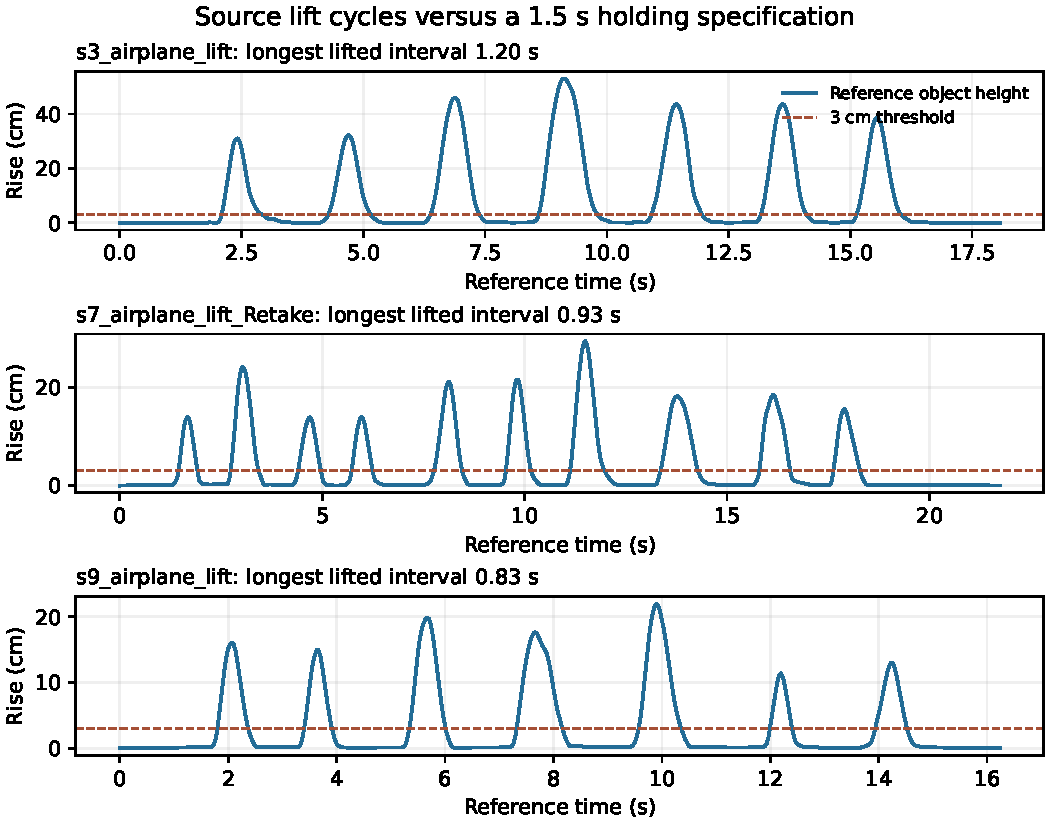
\includegraphics[width=.95\linewidth]{figures/reference_hold.pdf}
\caption{Source object-height targets over reference time. These are labels, not successful physical rollouts. Repeated lift/return cycles are incompatible with requiring perfect tracking and uninterrupted lift lasting 1.5 seconds simultaneously.}
\end{figure}

Eight historical native runs also have no retained success despite 70 stable
instances, including correlated repeats; the new trial has small positive
retained rates. Reference return does not prove the cause of every early drop.
The old gate remains failed. The experiment cannot establish that all predictive
control is useless or that every counted return is accidental object loss.
Repeated corrected states also differ from the first-contact contexts used to
fit this model. Both task specification and closed-loop distribution need attention.

Next we freeze an explicitly synthetic holding task: duplicate 90 raw reference
rows at the maximum height of each FIRST lifted interval, without selecting a
pose using simulator outcomes. The native loader recomputes velocities. A new
actor-only feasibility test asks for 75 consecutive contact-supported physical
steps in that inserted phase, before deliberate release. Generation preserves
initial rows and original remainder; it is not human-data or task-transfer evidence.
Completed results of the new task are reported separately below.

\section{Synthetic holding transfer and one frozen curriculum}
The three first-lift label peaks are frames 72/50/62. Inserting 90 identical raw
rows after each peak creates stationary phases 73--162, 51--140, 63--152, and
new reference lengths 633/743/578. All 598 columns are copied together; original
initial rows and remainder are preserved. The native loader recomputes all
velocity channels, independently verified zero throughout the plateau.

A separate feasibility gate requires 75 consecutive physical steps within the
90-row phase with root height at least 3 cm above its actual initial height and
both force proxies. It requires at least 10 percent pooled success and 5 percent
in every motion. Actual native progress, rather than collector-loop indices,
defines phase membership. Reference length and the complete first-episode endpoint
are independently checked; no early native episode is selected.

Actors 286/287 with fresh seeds 498/499 provide four 192-environment panels, 64 per
motion per panel. All 768 native episodes complete with actor/RMS frozen.
The original parent reporting stage fails on a duplicate keyword; physical files
are complete and preserved. A separate version uses the same frozen scoring
functions and independently reconstructs every label, without rerunning physics.
All 156 protected input hashes remain unchanged. Only 5/768 retained75 and 19/768
stable45 events occur; all four gates fail, UNPROMISING.

\begin{table}[h]
\centering
\begin{tabular}{lrrrrr}
\toprule
Screen & Motion & Episodes & Retained75 & Stable45 & Rise (mm)\\
\midrule
Actor transfer & 0 & 256 & 4 & 6 & -10.025\\
Actor transfer & 1 & 256 & 0 & 0 & 5.149\\
Actor transfer & 2 & 256 & 1 & 13 & 14.190\\
Actor transfer & Pooled & 768 & 5 & 19 & 3.105\\
PPO continuation & 0 & 128 & 0 & 0 & -1.703\\
PPO continuation & 1 & 128 & 0 & 0 & 3.906\\
PPO continuation & 2 & 128 & 0 & 0 & -1.396\\
PPO continuation & Pooled & 384 & 0 & 0 & 0.269\\
\bottomrule
\end{tabular}

\caption{Synthetic plateau episodes. Transfer and continuation use different cohorts and actor configurations; these rows are separate feasibility screens, not a matched treatment comparison.}
\end{table}

One separately frozen baseline continuation starts from self-trained actor 286's
fixed epoch 420 network and both observation statistics, with fresh optimizer and
new epoch count. Seed 721 receives exactly 300 new PPO epochs/460800 interactions:
96 environments, horizon 16, minibatch 512, four PPO passes, constant learning rate
0.00001. The final checkpoint alone is evaluated; no best/intermediate selection
or additional optimization seed is used. Wrist-translation exploration standard
deviation is predetermined at 5 mm; other coordinates retain their source values.

Half of training resets start at the first stationary row through epoch 80; this
probability decreases linearly to zero at epoch 200. The last 100 epochs all start
at frame 0. Native reference reward receives an additional bounded contact-supported
lift bonus of coefficient 10 only during the holding phase. There is no Cm,
action-selection teacher or other predictor. Training exposure is not success:
68947 plateau samples and 7933 positive bonus samples are privileged diagnostics.

The final checkpoint and evaluated model/statistics fingerprints match exactly;
all weights remain finite. Fresh seeds 500/501 each complete 192 first episodes.
No retained75 or stable45 instance occurs in 384 episodes; the force-proxy conjunction
is absent throughout the phase. All four gates fail, UNPROMISING. All 178 protected
inputs and independent trajectory labels pass closeout checks. This exact recipe
ends without extra epochs, seed or learning-rate tuning. The transfer and training
screens take 400.79/1120.95 seconds, respectively; one failed continuation does not
establish that self-training or all curricula are impossible.

\section{Native pose semantics and mechanical grip prerequisites}
The actual native reset method clamps and couples finger DOFs. A three-pose label
audit compares raw reference coordinates with that method applied to dummy tensors.
Maximum changes are 0.29677/0.26261/0.09957 rad. Sampled surface gaps change from
0.9135/0.9456/0.4883 mm to 0.3453/1.4025/0.8457 mm; geometric finger flags remain 3/1/1.
Thus reset changes do not explain failure through a demonstrated loss of these
minimum-proximity or binary-flag quantities. Unsigned proximity does not establish
nonpenetration or a compressive grasp.

A mechanical diagnostic bypasses the actor: initialize at the elevated zero-velocity
stationary row and hold the actual reset q as a constant absolute PD goal for 90
physical steps. Native action inversion is verified within2.981e-8; actor invocation
raises an error and model/statistics remain unchanged. Two fresh seeds 502/503 produce
192 complete trajectories. None satisfies 75 consecutive ticks of the necessary
height/proxy criterion: root at least 3 cm above original frame 0 and at most 1 cm below
its elevated initial height, with both force proxies. This is neither frame 0 pickup
nor proof of intrinsic grasp infeasibility.

The prospectively specified full-mesh table clearance contains a measurement error:
local Z was assumed the tabletop normal. The actual 21304-vertex table is thin along
local Y, and its native xyzw pose maps local -Y to world +Z. Original full-clearance
metrics are therefore INVALID\_TABLETOP\_AXIS and cannot support a physical-distance
claim. Original code, counts and failed gates remain intact. A separately recorded
offline correction uses all 25002 object vertices and the actual tabletop support
plane. Initial clearances are 307.03/130.93/153.56 mm. Independent NumPy world-up support
agrees within 0.000000118 m; corrected retained75 remains 0/192. This is explicitly
post-hoc reused-data geometry, not prospective Validation. The independently valid
necessary-condition failure does not depend on the mistaken clearance axis.

A followup saved-joint audit excludes another apparent issue: wrist rotations are
URDF continuous joints with no position bounds. A helper's default plus/minus pi
range is not a simulator hard limit. Motion 2 joint 5 at-4.59205 rad is tracked near
that value. All genuinely bounded goals satisfy their specified bounds. Nominal
PD-goal agreement must also be distinguished from realized tracking: maximal wrist
position deviations are 26.903/0.351/0.132 mm and finger deviations 0.0661/0.1940/0.0693 rad.
These observations do not identify the cause of grip failure.

A new prospective mechanical screen asks whether additional finger closure can
supply holding forces while keeping the wrist fixed. Doses 0/0.05/0.15/0.30 rad are
added to independent curl joints 6/8/10/12/15; thumb yaw 14 and wrist 0--5 are unchanged.
Each parent is capped by both its own and dependent native limits, then dependent
coupling is reconstructed. Initial physical q is unchanged; closure is an actuator
target at the first step, not a state teleport. Six overwritten command coordinates
remain canonical zero. No policy is invoked and no action is clipped.

Fresh seeds 504/505 each use 96 environments. Within each motion a private generator
randomly permutes eight copies of each dose before physics, giving 16 trajectories
per dose/motion overall. All 192 run 90 physical steps. The full retention criterion
is prospectively implemented with the correct thin tabletop geometry and independently
reconstructed world-up clearance, force proxies and longest runs. Each positive dose
must reach 50 percent pooled, 25 percent in every motion, and at least 25 percentage
points pooled gain over zero. Candidate dose screening is not formal Validation.

\begin{table}[h]
\centering
\begin{tabular}{lrrrr}
\toprule
Dose (rad) & Pooled /48 & Motion0 /16 & Motion1 /16 & Motion2 /16\\
\midrule
0.00 & 0 & 0 & 0 & 0\\
0.05 & 0 & 0 & 0 & 0\\
0.15 & 6 & 6 & 0 & 0\\
0.30 & 13 & 8 & 0 & 5\\
\bottomrule
\end{tabular}

\caption{Prospective bounded closure screen: retained75 counts at each dose. All dose gates fail; motion-specific counts are retained rather than replacing the pooled and every-motion criteria.}
\end{table}

No dose meets all gates, UNPROMISING. The 0.30 rad dose meets the gain requirement,
but its 27.08 percent pooled rate and zero success on motion 1 fail the other conditions.
Successful instances on motions 0/2 expose a concrete mechanical candidate signal,
without proving pickup, policy learning, force closure or generalization. This
exact four-dose family ends without larger-dose or selected-seed expansion.
The screen takes 76.99 seconds and 9.43 MiB; all 189 protected hashes remain unchanged.
Independent clearance disagreement is at most 0.000000482 m. The distinct next question
is grasp-pose construction and contact geometry, before another baseline learner. These statements describe the decision at that
screen; the subsequent frame 0 witness and independent learners appear below.

\begin{figure}[h]
\centering
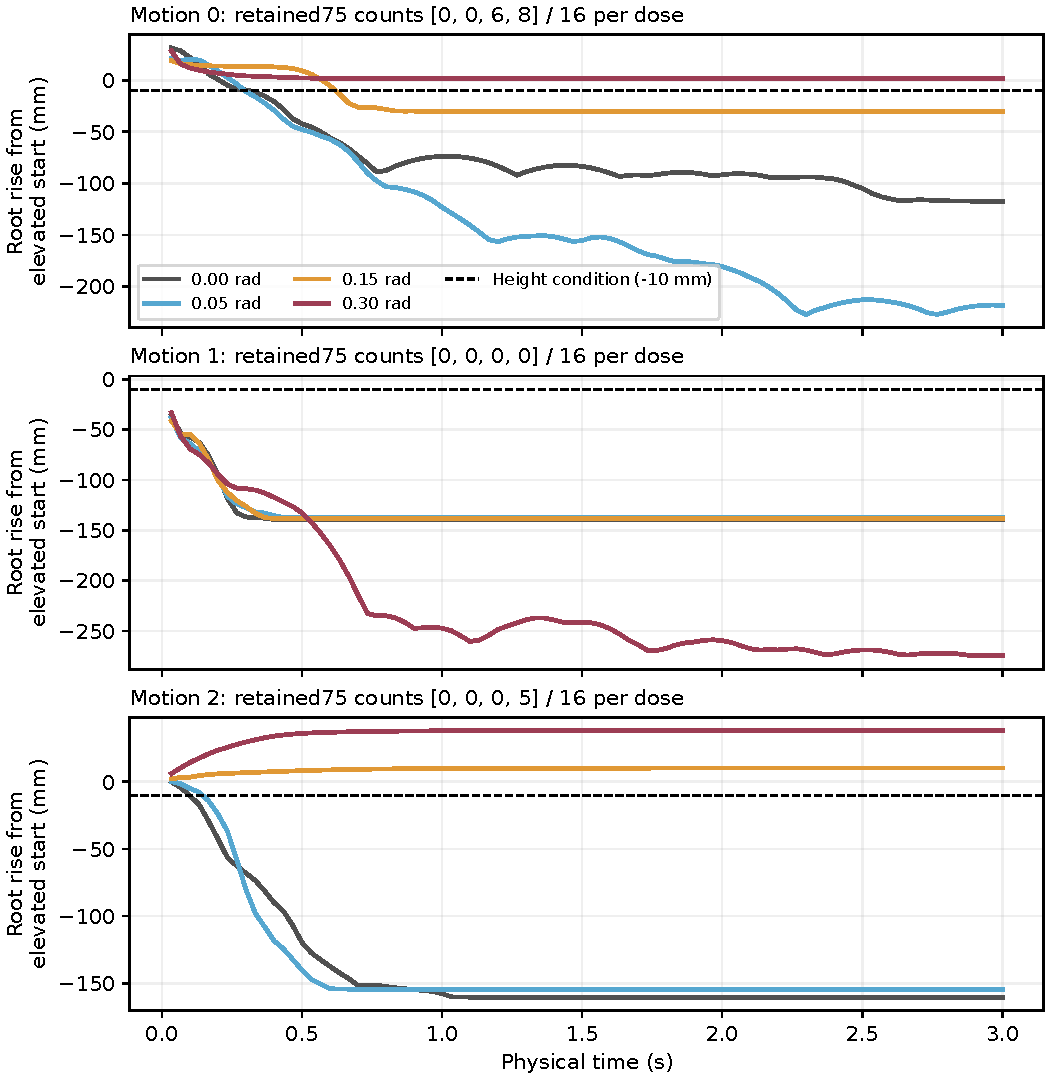
\includegraphics[width=.95\linewidth]{figures/finger_preload.pdf}
\caption{Physical object-root trajectories for the prospective closure screen. Each curve averages 16 trajectories per motion/dose. The dashed line is only the initial-height condition; forces, table clearance and 75 consecutive steps are additionally required. Mean height is not retained success or a policy benefit.}
\end{figure}

\section{Prospective support-removal witness}
An original-frame 0 tracking controller follows the available reference joint plan,
with a timed 0.30 rad curl increment, then holds the last plateau target. Its original
strict-force gate remains UNPROMISING: unchanged/closure counts 0/96 versus 5/96
on fresh 506/507. Geometry-only motion 1 retention 32/32 is explicitly secondary.
The actual object weighs 2.5936 g under native gravity; the 0.1 N net-body force
threshold is 3.93 times its weight. Neither this ratio nor geometry alone establishes
the hand's contribution, motivating a prospective removal experiment.

Before new physics, motion 1 is selected as the primary stratum. In each fresh
seed 508/509, 96 environments cover all three motions with 32 each. Private random
assignment balances 16 continued-hold and 16 release environments per motion.
All follow the same controller through the plateau stop. Release then commands
open fingers and 20 cm wrist retreat; controls retain their last target. All 202
physical ticks run with gravity, unmodified object state and three native actors.
The horizon is corrected from 200 to 202 before physics to cover every motion's
late window; primary motion 1 gates are unchanged. Warm solver-state clones are
not asserted. Five requirements per seed are fixed: at least 80 percent prior
geometry75 in each arm, 90 percent realized retreat of 15 cm, 80 percent control late
retention, 80 percent release late loss, and 30 mm mean height separation. The late
window is stop+30 through stop+40 inclusive, all 11 ticks required.

\begin{table}[h]
\centering
\begin{tabular}{lrrrrr}
\toprule
Seed & Prior hold & Prior release & Late hold & Late loss & Height (mm)\\
\midrule
508 & 16 & 16 & 16 & 16 & 147.113\\
509 & 16 & 16 & 16 & 16 & 144.379\\
\bottomrule
\end{tabular}

\caption{Prospective primary-motion support witness. Counts retain all 16 environments per arm and seed. Prior geometry75 precedes intervention; late loss/retention require all 11 late ticks. Height is control-minus-release mean in the late window.}
\end{table}

All ten predeclared gates pass, PROMISING as a mechanical Probe. Every release
achieves measured retreat; control late retention and release late loss are 32/32.
Motion 0/2 remain unsuccessful in both arms and are not excluded from the archive.
Historical strictforce75 counts are 47/64 on the 64 prior geometrically held primary
trajectories. This identifies disagreement for this verified setting, not a
universal force-proxy error rate. The intervention provides evidence of mechanical
support, not force closure or learned-policy competence. Runtime 102.35 s, 17.03 MiB,
all 193 protected inputs unchanged; independent full mesh clearance error 3.80e-8 m.

\begin{figure}[h]
\centering
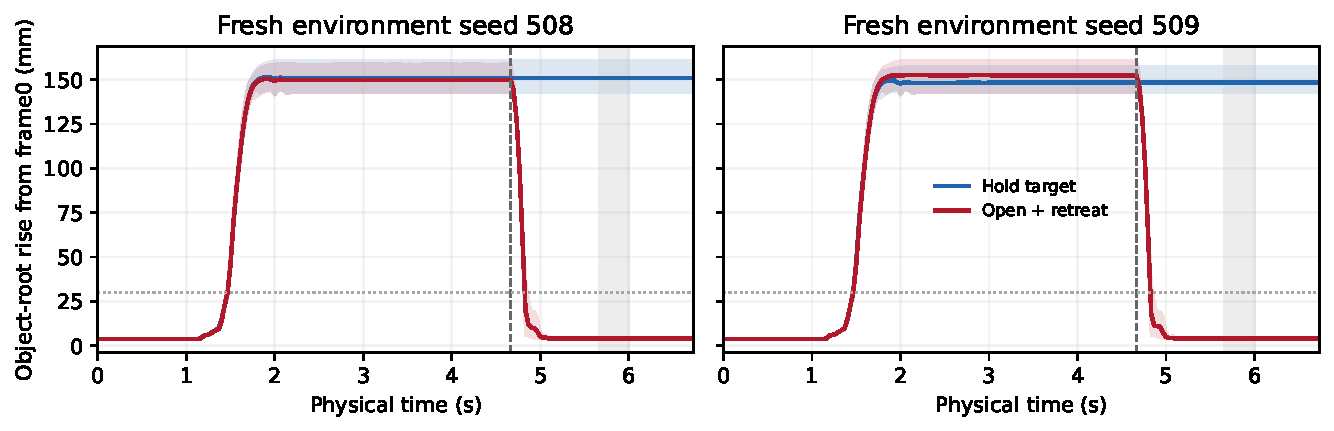
\includegraphics[width=.95\linewidth]{figures/support_removal.pdf}
\caption{Actual primary-motion object-root trajectories, all 16 assigned rows per curve. Bands show minimum/maximum across trajectories, not confidence intervals. Dashed vertical line marks intervention; shading marks the 11-tick late window. No learned actor controls these trajectories.}
\end{figure}

\section{Independent observation-policy learning}
The witness motivates a new prospective holding criterion: object-root rise from
actual frame 0 at least 30 mm and full mesh tabletop clearance at least 20 mm at every
tick from plateau-stop-74 through stop+30 inclusive. This 105-tick window includes
75 plateau ticks followed by 30 drop-checking ticks under the holding reference.
It does not relabel any historical failed gate. Strictforce 75 remains secondary.
Known motion 1 must reach 50 percent pooled and 25 percent in each fresh seed;
all three motions remain in training and reporting.

A random 512/256/128 ReLU/Tanh policy uses 70 features: current native joint position
and velocity, current object root state, two current force proxies, 18 planned joint
coordinates and planned phase fraction. Both teacher and actor have the planned
reference; no observed future state, teacher action or outcome enters the actor.
Seed 510 supplies all 19392 teacher rows. Fixed 2000 Adam updates, lr 0.001, batch 512,
weighted action errors and final-only checkpoint use FIT normalization. The six
hardware-null command coordinates are canonicalized. No source actor weights are
used; it is loaded solely for native environment construction and never called.
New 511/512 evaluations contain 192 complete 202-tick trajectories without fallback.
Physical 105 and strictforce75 are both 0/192, UNPROMISING. Training loss is not
manipulation success. Causal input and native PD reconstruction independently pass.

A separate descriptive saved-data diagnostic finds motion 1 late wrist-target
RMSE 170.58/171.36 mm; input normalization does not clip any motion 1 policy context.
Independent teacher-query reconstruction matches saved teacher targets. These
observations motivate, without establishing a causal explanation, one fixed
on-policy aggregation experiment. Fresh 513/514 collect only frozen-policy actions;
teacher labels are queried offline at visited states and never executed in these
cohorts. All original 19392 teacher rows and 38784 visited-state rows are retained.
No 511/512 test row is fitted. Baseline weights and normalization are preserved,
optimizer reset; sampling seed 735, 2000 updates and all other hyperparameters fixed.
Final-only evaluation uses new 515/516 seeds and the same physical105 gate.
The aggregation also fails both gates: physical105 and strictforce75 are 0/192,
including 0/64 on motion 1. The 184.70 s run preserves 217 protected inputs; this exact
aggregation ends without further rounds. Smaller posthoc wrist-target errors
do not replace the failed manipulation gate.

A distinct scratch actor changes the learned output to reference-relative absolute
PD targets. Residual scales are 20 mm for wrist translation, 0.10 rad for wrist
rotation and 0.40 rad for fingers. Targets enforce native bounds and coupling;
the exact native PD inverse supplies feedback from actual current joints.
Original 510 teacher rows alone train the 70-input network, seed 736, 2000 updates,
unit residual MSE and final-only evaluation. No timed curl schedule executes
in testing. New 517/518 produce 56/64physical105 on primary motion 1, 28/32 each seed,
passing both initializer gates: PROMISING. Motions 0/2 each remain 0/64;
pooled 56/192 and historical strictforce75 is 50/192. The 117.16 s run verifies all 226
protected inputs, causal context and independent residual-target/PD reconstruction.
This provides an initializer, not a reference-free actor, full multi-motion
competence or Cm benefit. Different losses, coordinates and physical cohorts
prevent a matched superiority claim over prior learners. All earlier failures
remain failed; baseline-only tuning stops here.

\begin{table}[h]
\centering
\begin{tabular}{lrrrr}
\toprule
Policy & Motion & Trajectories & Physical105 & Force75\\
\midrule
Scratch BC & 0 & 64 & 0 & 0\\
Scratch BC & 1 & 64 & 0 & 0\\
Scratch BC & 2 & 64 & 0 & 0\\
Scratch BC & Pooled & 192 & 0 & 0\\
One aggregation & 0 & 64 & 0 & 0\\
One aggregation & 1 & 64 & 0 & 0\\
One aggregation & 2 & 64 & 0 & 0\\
One aggregation & Pooled & 192 & 0 & 0\\
Absolute target & 0 & 64 & 0 & 0\\
Absolute target & 1 & 64 & 56 & 50\\
Absolute target & 2 & 64 & 0 & 0\\
Absolute target & Pooled & 192 & 56 & 50\\
\bottomrule
\end{tabular}

\caption{Independent learned-policy evaluations: physical105 is the new prospective primary and strictforce75 is a historical secondary. All variants retain all three motions. These are initializer Probes, without Cm or policy-training utility claims.}
\end{table}


\section{Executable support prediction and strong global controls}
The scratch reference-target actor is frozen. A new distribution independently
perturbs initial object XY within plus/minus 10 mm before the first counted physical
tick. It leaves initial height, orientation, velocity, mass and gravity unchanged.
Within each motion, eight executable target changes are balanced before physics:
unchanged, shared curl changes of -0.30/-0.15/+0.15 rad, or worldX/Y target changes
of plus/minus 10 mm. Changes start eight ticks before reference lift and persist
under the frozen learned actor. Native PD targets are recalculated each tick;
commands are not numerical open-loop action replay.

An initial engineering run fails before controlled physics because a GPU state
refresh immediately follows deferred reset setters. Its failed artifacts remain
retained. A new frozen implementation queues native root/DOF resets and commits
each combined setter once before the first simulate call. Immediate refreshes
are suppressed, and every subsequent state/force write is prohibited. All 6144
new trajectories complete 202 ticks; initial packets, native targets and geometric
outcomes are independently reconstructed. Full-mesh support extrema are audited
using a convex hull checked against all 25002 vertices, with maximum clearance
disagreement 3.20e-7 m. This corrects an implementation, not a scientific outcome.

FIT 519--524 contains 4608 rows; TEST 525/526 contains 1536. One pre-intervention row
contains 69 current physical/reference features and three primitive parameters.
Two matched 72-input 64/64 ReLU models share initialization 741 and 1000 Adam updates,
batch 256, learning rate 0.001, final checkpoint only and FIT-only normalization.
Cm receives primitive parameters; the state control receives three zero slots.
A strong privileged motion/action control estimates Beta-smoothed FIT frequencies.
The primary physical30 event requires root rise at least 30 mm and entire-mesh
table clearance at least 20 mm for all last 10 ticks of the next 30. It is a short
physical forecast under this continuation, not a long-term action value.

\begin{table}[h]
\centering
\begin{tabular}{lrrr}
\toprule
Cohort & Cm log loss & State log loss & Global log loss\\
\midrule
Motion1 & 0.122155 & 0.611316 & 0.130897\\
Motion1 seed525 & 0.141556 & 0.612498 & 0.142789\\
Motion1 seed526 & 0.102755 & 0.610134 & 0.119004\\
All motions & 0.093218 & 0.295303 & 0.182906\\
\bottomrule
\end{tabular}

\caption{Frozen forecast log losses; smaller is better. Motion 1 is preselected. All-motion results are secondary and do not replace the primary gate.}
\end{table}

Primary motion 1 has 364/512 physical30 positives. Cm improves log loss 80.02\% against
state-only but 6.68\% against the global control, below the required 10\% against BOTH.
Class diversity and per-seed improvement gates pass; the primary remains UNPROMISING.
All-motion physical105 is 370/1536, separately audited: motion 0/1/2 counts 0/304/66.
No extra updates or subgroup replacement follow. Neither short forecast loss nor
these physical outcomes demonstrate matched trained-policy utility.

\section{Corrected-gradient and positional headroom screens}
The next distinct cheap question uses the frozen predictors and already inspected
TEST rows to study corrected gradient noise for actual physical105 reward.
This is explicitly posthoc/reused-data exploration. Control variates and expected
finite-action gradients are established by Q-Prop, expected policy gradients and
related doubly robust policy-gradient work \cite{gu2017,ciosek2020,huang2020}.
Our algebra is an application, not a new theorem. With known behavior propensity
one-eighth, the sampled importance-weighted score times reward minus frozen
prediction is corrected by the exact eight-action expectation of score times
prediction. For any fixed prediction, the model terms cancel in expectation.
Thus short-horizon predictions need not equal the longer reward to form a valid
fixed control variate; that identity does not make them long-term values.

A fixed seed 751 trunk with 69 inputs and 64/64 hidden layers precedes a zero-weight
8-logit head, with bias 2 for unchanged and 0 otherwise. All 520 active head-gradient
coordinates are included. At this initializer, earlier-layer gradients are zero.
Coefficient 1 is fixed. Population mean gradients agree under the randomized design,
so second-moment DIFFERENCES identify gradient-variance differences. Finite observed
mean differences are reported without asserting population equality from the sample.

\begin{table}[h]
\centering
\begin{tabular}{lrrr}
\toprule
Cohort & Cm moment & State moment & Global moment\\
\midrule
All motions & 0.231475 & 0.284534 & 0.274234\\
Seed525 & 0.220441 & 0.259844 & 0.277084\\
Seed526 & 0.242508 & 0.309224 & 0.271384\\
\bottomrule
\end{tabular}

\caption{Full-gradient squared-norm means from 1536 reused rows. Absolute second moments are not themselves identified gradient variance or policy utility.}
\end{table}

Cm lowers pooled moments 18.65\% versus state-only and 15.59\% versus global, failing
the fixed 20\% gate against BOTH. Per-seed reductions pass. The candidate is
UNPROMISING and ends without coefficient or actor-seed selection. Independent
NumPy reduction agrees within 2.22e-16; assigned probabilities replay exactly and
finite-action cancellation tests pass. No model refitting or physical training
occurs in this screen, and the preceding failed forecast gate remains failed.

A separate fixed structural benchmark asks whether current object-minus-native
translation XY can change the best primitive. FIT-only medians define four bins
per motion; Beta-smoothed FIT physical105 frequencies select bin-specific and
global arms. There is no feature/bin scan. On the same reused TEST cohort,
known randomized propensity yields Horvitz--Thompson fixed-policy estimates.
These are exploratory off-policy estimates, not executed policy success rates.

\begin{table}[h]
\centering
\begin{tabular}{lrrr}
\toprule
Cohort & Position IPW (%) & Global IPW (%) & Unchanged IPW (%)\\
\midrule
All motions & 34.375 & 38.021 & 32.812\\
Seed525 & 33.333 & 40.625 & 32.292\\
Seed526 & 35.417 & 35.417 & 33.333\\
\bottomrule
\end{tabular}

\caption{Position-bin headroom screen. All three motions and complete test cohorts retained; reported IPW estimates do not establish executed or learned-policy gains.}
\end{table}

The position policy is 3.65 percentage points below global and 1.56 above unchanged,
failing both predeclared criteria. This exact four-bin recipe is UNPROMISING,
without excluding all possible state dependence. Three failed candidate gates
close the nominal eight-primitive / initial-XY family rather than motivate an
unbounded local representation or hyperparameter sweep.

\section{Post-lift disturbance task calibration}
A new finite mechanical Probe checks whether already lifted objects have a
recoverable decision under disturbance. This explicitly changes the task
variant; prior physical30/105 gates stay unchanged. Initial XY is unperturbed.
Seeds 527/528 retain 1536 trajectories, with 32 balanced cells per motion: four issued
loads 0/0.05/0.15/0.45 N, two worldX directions and four recovery arms. Exactly one
step of force is issued to the object center of mass, without torque, at plateau
anchor plus 10. All other force tensor entries and ticks are zero. Object SDK
body indices and tensors are independently checked. No object root or velocity
reset follows initial placement. Actual contacts oppose the force; force times
step divided by mass is not an observed free-flight velocity change.

One tick later, the frozen actor continues unchanged, follows the known force
direction with 20 mm wrist target offset, opposes it, or applies 0.15 rad extra curl.
Direction-aligned arms are privileged mechanical probes, not learned deployable
policies. Prior geometry10 checks the preceding ten ticks. New recovery90 requires
at least 30 mm root rise and 20 mm whole-mesh clearance on all 90 ticks from stop minus 59
through stop plus 30, allowing a bounded transient before this window. It cannot
replace older failed holding criteria.

\begin{table}[h]
\centering
\begin{tabular}{lrrrrr}
\toprule
Load (N) & Prior /128 & Null /32 & Follow /32 & Oppose /32 & Curl /32\\
\midrule
0.00 & 128 & 32 & 32 & 32 & 29\\
0.05 & 128 & 32 & 32 & 32 & 26\\
0.15 & 128 & 32 & 32 & 32 & 27\\
0.45 & 128 & 30 & 31 & 31 & 25\\
\bottomrule
\end{tabular}

\caption{Primary-motion mechanical calibration. Counts are actual executed trajectories; no Cm or policy training occurs. All other motions and both seeds are also reported in the retained results.}
\end{table}

All primary trajectories have prior geometry10. Yet no nonzero load meets the
required unchanged 10--80\% recovery range or 15/10 percentage-point recovery contrasts.
At 0.45 N, unchanged holds 30/32; following and opposing each 31/32. No load is
eligible under the frozen lowest-eligible rule: UNPROMISING. The experiment
completes 115.44 s, all 248 protected inputs match, and independent clearance error
is at most 8.43e-7 m. End this exact force/axis/window recipe without further scans.
This does not refute disturbance recovery or Cm generally. Learned dynamics
planning, robust contact/motion recovery and contact-aware planning are already
established \cite{nagabandi2020,jiang2025,suh2026}; another calibration task alone
cannot supply a distinctive method.


\section{Matched return-trained physical-feature policies}
This is the first prospective trained-policy utility comparison on this track,
rather than a forecast-loss or frozen greedy-selection screen. Code
\texttt{34f78b6} freezes the scratch reference-target base actor and physical
predictors. Three identical 77-input, two-hidden-layer macro policies receive
current state plus eight Cm physical30 probabilities, repeated state-only
probability, or privileged FIT motion/action means. All share seed752, initial
weights and probabilities, optimizer, state-only return baseline and data.
Global controls execute the same neural queries before substituting FIT means.

Twelve fresh randomized panels529--540 provide9216 native trajectories. After
each panel, each policy receives exactly one full-batch importance-weighted score
update with actual physical105 reward, behavior probability1/8 and an
ACTION-INDEPENDENT FIT motion baseline. Adam learning rate0.01, two64-unit ReLU
layers, gradclip10 and12updates are fixed. There is no predicted reward, actor
weight transfer from the official model, extra replay or checkpoint selection.
Final-only evaluation541/542 assigns four balanced policy groups before physics;
trained heads choose deterministic argmax once at the pre-lift decision.

\begin{table}[ht]\centering
\begin{tabular}{lrrrr}
\toprule
Cohort & Initializer & Cm & State only & Global\\
\midrule
All /384 & 131 & 151 & 153 & 140\\
Seed541 /192 & 62 & 79 & 77 & 70\\
Seed542 /192 & 69 & 72 & 76 & 70\\
Motion0 /128 & 0 & 0 & 0 & 0\\
Motion1 /128 & 114 & 113 & 105 & 111\\
Motion2 /128 & 17 & 38 & 48 & 29\\
\bottomrule
\end{tabular}

\caption{Fresh physical105 counts for executed policies. Each all-motion policy
has384 trajectories; each seed192 and each motion128. All motions are retained.
Single optimization seed: exploratory Probe only.}
\end{table}

Cm151/384 versus state153/384 and global140/384 gives minus0.521 and plus2.865
percentage points. The frozen requirement of at least5 percentage points against
BOTH controls fails, as does each-seed noninferiority: UNPROMISING. Querying all
three saved head outputs on every one of1536 pre-decision states shows identical
argmax actions: unchanged on motions0/1, curl+0.15rad on motion2. The tested
executable decision rules coincide; unequal counts on different randomized
cohorts do not demonstrate a Cm-specific advantage. This observed agreement
neither proves stochastic-policy equivalence nor covers unseen states.

All14 native panel audits and12 independent NumPy score-gradient/Adam audits
pass. The parent remains FAILED solely at final analysis: a25nm independently
reconstructed clearance discrepancy was amplified by normalization and mistakenly
checked as same-input arithmetic. Separately retained analyzer\texttt{db96433}
first checks raw reconstruction, then replays actual saved native inputs with the
ORIGINAL tolerances. No resimulation, retraining, outcome edits or threshold
change. Corrected maximum raw/feature/logit errors are2.49e-8m,1.06e-6 and7.52e-6;
actual macro argmax agrees exactly. All374 parent input hashes are reverified.

This is established frozen-feature contextual policy learning, not a distinctive
algorithm. Physical predictor pretraining4608 trajectories and base teacher19392
rows are reported separately from9216 policy-training trajectories; no total
sample or compute saving is claimed. Stop this exact recipe without additional
updates, learning-rate/head/seed selection or altered deployment. Future work
must establish physical decisions beyond a per-motion constant action before
investing in another policy-training comparison.


\section{Natural support loss and prospective feedback feasibility}
A separately labeled training-only diagnostic retains all1152 unchanged-arm
trials from twelve randomized panels529--540. Motion0never acquires five
consecutive lifted ticks; motion1has56/384 and motion2has101/384 cases that
acquire then fail physical105. Every such case shows object-minus-hand downward
speed before first loss. Five-tick acquisition is only a diagnostic, never a
replacement success criterion; no evaluation data or learned model is used.

Code\texttt{7e2c741} freezes a new prospective native experiment543/544. All1536
trajectories retain original initial-XY variation, reference-conditioned scratch
base,202ticks, material/mass/gravity and physical105. Four privately preassigned
policies are unchanged, early curl+0.15rad at lift_start-8, event curl+0.15rad,
and event wrist-XYZ arrest. Before each action, a current-state trigger latches
five consecutive physically lifted ticks from lift_start, then fires once while
still lifted when object-minus-hand vertical velocity is at most-20mm/s. Event
curl persists; wrist arrest holds the measured translation at trigger while
orientation and fingers continue the base policy. No object/hand state writes,
external forces or future outcomes enter this controller.

\begin{table}[ht]\centering
\begin{tabular}{lrrrr}
\toprule
Cohort & Unchanged & Early curl & Event curl & Wrist arrest\\
\midrule
All /384 & 133 & 96 & 92 & 125\\
Seed543 /192 & 68 & 48 & 40 & 65\\
Seed544 /192 & 65 & 48 & 52 & 60\\
Motion0 /128 & 0 & 0 & 0 & 0\\
Motion1 /128 & 111 & 67 & 71 & 107\\
Motion2 /128 & 22 & 29 & 21 & 18\\
\bottomrule
\end{tabular}

\caption{Prospective natural-retention physical105 counts. Each pooled policy
has384 trajectories, each seed192, and each motion128. All trajectories and the
original criterion are retained; no event-conditioned subgroup replaces the
primary. These are mechanical controller results, not Cm training.}
\end{table}

Event curl92/384 trails unchanged133/384 by10.677 percentage points. Wrist
arrest125/384 trails unchanged by2.083 points, although it exceeds harmful early
curl96/384. Neither satisfies the predefined5-point gain over BOTH controls or
each-seed noninferiority: UNPROMISING. Complete independent NumPy event timing,
current state, native target/PD, private assignment and full-mesh labels pass;
maximum clearance error2.607e-7m. Run completes114.312s,271742088bytes; all251
protected input hashes are rechecked. Stop the exact trigger/action family
without threshold, dose, axis or timing scans.

Observability does not establish intervention value in this setting. Unchanged
motion1has82 successful and17 failed trajectories that trigger; motion2has10
successful and39 failed triggering trajectories. Relative downward speed need
not imply that more closure or wrist arrest helps. Early curl changes the
pre-event physical prefix, so event-conditioned cross-policy rates are not
matched causal comparisons. Root pose/velocity and joint state are privileged
simulator observations; no sensing or hardware transfer is demonstrated.

Slip-direction grasp reflexes are already established\cite{abd2018}. Predictive
and reactive tactile residuals\cite{zhou2026}, action-conditioned pre-contact
failure monitoring\cite{zheng2026}, and causal temporal detectors with conformal
alarm calibration\cite{zhang2026} also precede this screen. A generic
forecast-plus-feedback design is insufficient for a distinctive method. The
next decision concerns independent effective finger actions: common curl can
harm successful contacts, while a visible loss cue does not specify a useful
correction. Selective-actuator feasibility still would not establish Cm utility;
a subsequent method requires matched actual policy learning and Validation.

\section{Selective independent-finger feasibility}
After the failed slip-reflex screen, we test whether the common curl synergy
conceals useful independent corrections. The native SDK and the read-only
Inspire URDF agree on six effective coordinates: index 6, middle 8, pinky 10,
ring 12, thumb yaw 14 and thumb curl 15. Children 7/9/11/13/16/17 are reconstructed
from parent commands and are not independent policy dimensions. This action
accounting is an implementation prerequisite, not a new modeling method.

Two fresh seeds, 545 and 546, provide 1536 native trajectories of 202 ticks each.
Before physics, eight arms are independently randomized within each motion:
32 trials per arm, motion and seed. We retain the same base actor, references,
private initial XY offsets and physical105 criterion. At eight ticks before
lift start, we persist either no correction, shared curl (+0.15 rad on
coordinates 6/8/10/12/15), or a single +0.15 rad correction on one of
6/8/10/12/15/14. Wrist targets are unchanged. Requested offsets and actual
bounded target offsets are recorded separately; dependent and native limits
are independently reconstructed. The preselected motion 2 gate requires at
least 20 percentage-point gain over both unchanged and common curl, with no
loss to either control in each seed. The six selective candidates constitute a
declared mechanical screen, not a fitted policy or formal validation.

\begin{table}[ht]
\centering
\begin{tabular}{lrrrr}
\toprule
Arm & Motion 0 /64 & Motion 1 /64 & Motion 2 /64 & All /192\\
\midrule
Unchanged & 0 & 54 & 12 & 66\\
Shared curl & 0 & 39 & 21 & 60\\
Index & 0 & 39 & 10 & 49\\
Middle & 0 & 45 & 6 & 51\\
Pinky & 0 & 55 & 10 & 65\\
Ring & 0 & 56 & 6 & 62\\
Thumb curl & 0 & 54 & 8 & 62\\
Thumb yaw & 0 & 53 & 4 & 57\\
\bottomrule
\end{tabular}

\caption{Fresh selective-finger physical105 counts from all 1536 trajectories. Each motion has 64 trials per arm; pooled counts have 192 per arm. Motion 2 is the preselected primary. Every fixed selective-correction gate fails.}
\end{table}

\begin{figure}[ht]
\centering
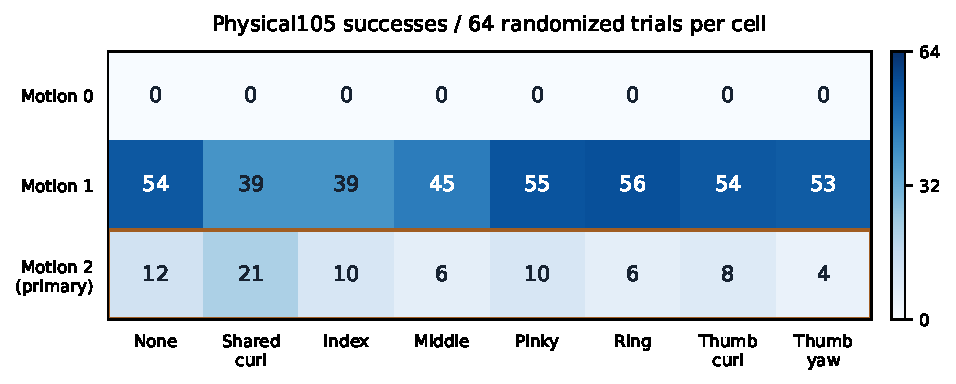
\includegraphics[width=\linewidth]{figures/selective_fingers_heatmap.pdf}
\caption{Recorded physical105 successes for all eight prospective arms in every motion. The outline identifies the preselected primary. This fixed mechanical screen measures no learned Cm policy performance, and no subgroup replaces the failed primary gate.}
\end{figure}

Motion 2 gives 12/64 successes for the unchanged actor and 21/64 for common curl;
selective arms yield 4--10/64. All primary candidate gates fail, UNPROMISING.
The run completes in 112.349 s and retains 279708481 bytes; all 255 protected
inputs and full-mesh, current-state, native-PD and assignment audits pass.
Independent clearance error is at most 0.000222 mm. This closes the exact
positive-offset family without sign, dose or timing scans. It does not rule out
continuous feedback learning, negative adjustments or other task distributions.

At the first intervention in motion 1, requested thumb yaw is target-null in
64/64 trials and thumb curl in 47/64; both encounter bounds in 64/64.
These current command/limit diagnostics are not future measured hand motion,
whole-trajectory counterfactuals, or evidence that unused dimensions can never
matter. Independent randomized cohorts do not identify interaction effects
between combined fingers.

\section{Continuous policy comparison: implementation evidence only}
We separately freeze a full 12-coordinate continuous PPO comparison: a Cm
physical auxiliary critic, a state-only auxiliary control and a no-auxiliary
control, with identical initial actor/critic parameters and equal native
interactions. The value baseline remains state-only. Cm's auxiliary head
receives current state and actual executable target minus current joint
position, and predicts the next object position and linear-velocity change.
Separate actor and critic encoders prevent auxiliary gradients from directly
updating the actor. The only task reward is actual terminal physical105,
not predicted reward or a success surrogate.

Gaussian request likelihood is computed before tanh and native projection;
it is not an executable-target density or entropy. Auxiliary actor-critic
objectives are established \cite{jaderberg2016}. Replacing clipped request-tail
scores with boundary probability mass substantially overlaps CAPG
\cite{fujita2018}. Neither operation is claimed as a new contribution.

The 768-trajectory engineering panel (seed 567) passes independent current-state,
projection, likelihood, critic and one-step physical-target audits with zero
optimizer updates. Subsequent fresh training on seed 547 completes one matched
update and all three predetermined first-minibatch gradient/Adam audits.
Native collection on seed 548 is independently audited after the execution
environment changes. This partial training has no final evaluation and no
policy-utility label. The frozen design still requires 20 training panels
(seeds 547--566) and final-checkpoint-only evaluation on seeds 568/569.
Training losses and subset success rates cannot replace this incomplete
comparison. The journal objective remains active.

\section{Limitations and research decision}
These experiments involve one object, three shared motions, two existing actors
and small fixed fitting procedures. Contact proxies plus sampled proximity are
not attributed pairwise forces. Short-horizon measurement is not stable lift,
retention or manipulation utility. One fixed baseline PPO continuation is presented; The first matched frozen-feature policy-training comparison is negative;
unseen-object/hand evaluation and hardware deployment remain absent. Optimization seeds do not create independent
physical datasets. Existing papers' claims are not replaced by these diagnostic tests.

The direct learner and tested greedy controller are stopped at their fixed gates.
The reference-target initializer supports bounded physical studies, but the
subsequent forecast, gradient, position and finite-disturbance candidates fail.
Matched Cm-on/off POLICY TRAINING has now been executed without utility;
meaningful conditional decision headroom is the consequential next requirement. A compatible reference is a
prerequisite, not proof of controllable contact or model benefit. Synthetic plateau transfer, one fixed continuation and mechanical feasibility
screens are completed with their original failed gates retained. Corrected geometry
is labeled explicitly as a separate reused-data diagnostic.

The original user objective remains a journal-level research outcome. This working
paper does not meet it: a distinctive method and consequential matched task evidence
remain necessary. Negative outcomes and unresolved policy utility are retained
to guide further work rather than converted into positive conclusions.

\section*{Reproducibility}
All new work is isolated in branch \texttt{agent/contact-response-cm}. Original
checkpoints, motion assets and prior evidence are read-only. Physical/differential
code is fixed at \texttt{466e80d}/\texttt{44f22ea}; factorization at
\texttt{bbd5ba4}; fresh collection at \texttt{59de1cf}; null recovery at
\texttt{33d1085}. Randomized collection uses \texttt{510a00e}; direct fitting
\texttt{2075314}; independent auditing \texttt{f283bb9}. Closed-loop task
collection uses \texttt{c0ec955}; task/reference audit and next synthetic task
design use \texttt{b2b26e0}. Holding collection/corrected reporting use
\texttt{40e73f2}/\texttt{3f4ae77}; the frozen continuation uses \texttt{e770d4b}.
Native reset/static diagnostics use \texttt{da39660}/\texttt{1e38cf6}; the independent
geometry correction uses \texttt{68bf178}; prospective finger closure uses \texttt{5d7c375}. Frame 0 tracking uses \texttt{d15ef0f},
support witness \texttt{49cf8b3}, scratch observation policy \texttt{9c0a218}, and
fresh corrective-label aggregation \texttt{e2a38c2}, reference-target actor \texttt{596c5a0}.
Executable support forecasting/reset correction use \texttt{5140208}/\texttt{3ac4f6c};
corrected-gradient screen \texttt{ef71c33}, positional screen \texttt{f66aa01},
and one-step physical disturbance calibration \texttt{721b44d}.
Manifests preserve commands, input SHA, GPU UUID,
budgets and failures. The first feature-policy comparison uses code\texttt{34f78b6}; its separately
retained final audit correction uses\texttt{db96433}.
Every table and figure comes from recorded labels or physical trajectories, clearly distinguished.
The PDF is a ReportLab review copy; portable LaTeX source and tables are also
retained. Earlier manuscript revisions are preserved separately.


\begin{thebibliography}{24}
\bibitem{he2025} Z.He et al. Scaling Cross-Embodiment World Models for Dexterous Manipulation.
arXiv:2511.01177, 2025. \url{https://arxiv.org/abs/2511.01177}.
\bibitem{xu2025} S.Xu et al. Dexplore:Scalable Neural Control for Dexterous Manipulation
from Reference-Scoped Exploration.2025. \url{https://arxiv.org/abs/2509.09671}.
\bibitem{farahmand2017} A.-M.Farahmand, A.Barreto, D.Nikovski. Value-Aware Loss Function
for Model-based Reinforcement Learning.2017. \url{https://proceedings.mlr.press/v54/farahmand17a.html}.
\bibitem{qiu2026} J.Qiu et al. AD-WM:Action-Discriminative World Models for Counterfactual
Model Predictive Control.2026. \url{https://arxiv.org/abs/2609.30264v2}.
\bibitem{rudolph2024} M.Rudolph et al. Learning Action-based Representations Using Invariance.
2024. \url{https://arxiv.org/abs/2403.16369}.
\bibitem{fey2026} N.Fey et al. Contact-UAN:Unsupervised Actuator Networks as a Residual
World Model for Humanoid Control.2026. \url{https://contact-uan.csail.mit.edu/}.
\bibitem{rakelly2021} K.Rakelly, A.Gupta, C.Florensa, S.Levine. Which Mutual-Information
Representation Learning Objectives are Sufficient for Control?2021.
\url{https://arxiv.org/abs/2106.07278}.
\bibitem{yuan2026} H.Yuan et al. DexTacWAM:A Visuo-Tactile World-Action Model for
Dexterous Manipulation.2026. \url{https://arxiv.org/abs/2609.24976v1}.
\bibitem{yin2026} J.Yin et al. How to Learn from What a Human Would Avoid?
Intervention-Aware World Models with Real-World RL for Dexterous Manipulation.2026.
\url{https://arxiv.org/abs/2609.06009v1}.
\bibitem{qin2026} Y.Qin et al. DexTouch-WM:Learning Action-Conditioned Tactile World
Models from Human Touch for Dexterous Robot Manipulation.2026.
\url{https://arxiv.org/abs/2609.20649v2}.
\bibitem{co2026} P.Co et al. WorldSimProbe:Diagnosing Simulator Faithfulness in
Action-Conditioned World Models for Embodied Manipulation.2026.
\url{https://arxiv.org/abs/2608.09298v1}.
\bibitem{deng2026} H.Deng et al. Facet-0:A Robotic Foundation Model for Contact-Rich
Precise Manipulation.2026. \url{https://arxiv.org/abs/2609.01596v1}.

\bibitem{gu2017} S.Gu et al. Q-Prop: Sample-Efficient Policy Gradient with an Off-Policy Critic. ICLR2017. \url{https://arxiv.org/abs/1611.02247v3}.
\bibitem{ciosek2020} K.Ciosek, S.Whiteson. Expected Policy Gradients: A General Framework. JMLR2020. \url{https://arxiv.org/abs/1801.03326v2}.
\bibitem{huang2020} J.Huang, N.Jiang. From Importance Sampling to Doubly Robust Policy Gradient. ICML2020. \url{https://proceedings.mlr.press/v119/huang20b.html}.
\bibitem{nagabandi2020} A.Nagabandi et al. Deep Dynamics Models for Learning Dexterous Manipulation. CoRL/PMLR100,2020. \url{https://proceedings.mlr.press/v100/nagabandi20a.html}.
\bibitem{jiang2025} Y.Jiang et al. Robust Model-Based In-Hand Manipulation with Integrated Real-Time Motion-Contact Planning and Tracking.2025. \url{https://arxiv.org/abs/2505.04978}.
\bibitem{suh2026} H.J.T.Suh et al. Dexterous contact-rich manipulation via the contact trust region. IJRR2026. \url{https://journals.sagepub.com/doi/10.1177/02783649251398875}.

\bibitem{abd2018} M.A.Abd, I.J.Gonzalez, T.C.Colestock, B.A.Kent, E.D.Engeberg.
Direction of Slip Detection for Adaptive Grasp Force Control with a Dexterous
Robotic Hand. IEEE/ASME AIM2018. \url{https://pmc.ncbi.nlm.nih.gov/articles/PMC7009943/}.
\bibitem{zhou2026} J.Zhou et al. TouchWorld: A Predictive and Reactive Tactile
Foundation Model for Dexterous Manipulation.2026. \url{https://arxiv.org/abs/2607.07287v2}.
\bibitem{zheng2026} G.Zheng, M.Johnson-Roberson, W.Zhi. ContactGuard: Pre-Contact
Execution Monitoring with Action-Conditioned Latent World Models.2026.
\url{https://arxiv.org/abs/2608.13438v1}.
\bibitem{zhang2026} H.Zhang et al. Foresight: Failure Detection for Long-Horizon
Robotic Manipulation with Action-Conditioned World Model Latents.2026.
\url{https://arxiv.org/abs/2606.23085v1}.
\bibitem{jaderberg2016} M.Jaderberg et al. Reinforcement Learning with Unsupervised Auxiliary Tasks.2016. \url{https://arxiv.org/html/1611.05397}.
\bibitem{fujita2018} Y.Fujita, S.Maeda. Clipped Action Policy Gradient. ICML/PMLR80:1597--1606,2018. \url{https://proceedings.mlr.press/v80/fujita18a.html}.
\end{thebibliography}
\end{document}
